% The 2026-2027 AIDaS Seed Grant proposal: cover (1 page), narrative (3), alignment (1), budget (1), biosketches.
% pdflatex alone builds it; on Overleaf, upload the zip of this folder and compile main.tex.
% contacts.tex and biosketch_han.pdf / biosketch_schwiebert.pdf are read when they sit beside this file and are
% never committed (root CLAUDE.md rule 12): without them the cover shows placeholders and the last page says
% where the biosketches go. Red [DATA NEEDED] marks are the investigators' to fill before submission.
\documentclass[10pt,letterpaper]{article}

\usepackage[T1]{fontenc}
\usepackage[utf8]{inputenc}
\usepackage{helvet}
\renewcommand{\familydefault}{\sfdefault}
\usepackage{sansmath}
\sansmath
\usepackage[letterpaper,margin=0.7in,footskip=0.3in]{geometry}
\usepackage{graphicx}
\usepackage{array,booktabs,tabularx}
\usepackage{xcolor}
\usepackage{enumitem}
\usepackage{titlesec}
\usepackage[font=footnotesize,labelfont=bf,labelsep=period,skip=3pt]{caption}
\usepackage{microtype}
\usepackage{pdfpages}
\usepackage{multicol}
\usepackage[hidelinks]{hyperref}
\hypersetup{pdftitle={Self-Repairing AI Agents on the Wayne State Grid: AIDaS Seed Grant 2026-2027}}

\definecolor{ink}{HTML}{1D1D1B}
\definecolor{teal}{HTML}{0F5F55}
\definecolor{rule}{HTML}{C9C5BA}
\definecolor{tbdred}{HTML}{B3261E}
\color{ink}

\newcommand{\tbd}[1]{{\color{tbdred}[DATA NEEDED: #1]}}
\newcommand{\aim}[1]{{\color{teal}\bfseries #1}}
\newcommand{\pct}{\,\%}

\IfFileExists{contacts.tex}{\input{contacts.tex}}{% Contact lines for the cover page. The submitted copy reads contacts.tex instead, which is never committed
% (root CLAUDE.md rule 12): copy this file to contacts.tex beside main.tex and fill in each line.
% Each line is LaTeX, so write a percent sign as \%, an underscore as \_ and an ampersand as \&: an e-mail address
% with an underscore in it stops the build until its underscore is written \_.
\newcommand{\HanContact}{Contact: \tbd{office, phone and e-mail}.}
\newcommand{\SchwiebertContact}{Contact: \tbd{office, phone and e-mail}.}
}

\setlength{\parindent}{0pt}
\setlength{\parskip}{2.5pt}
\titleformat{\section}{\normalfont\large\bfseries}{}{0pt}{}
\titlespacing*{\section}{0pt}{0pt}{3pt}
\titleformat{\subsection}{\normalfont\normalsize\bfseries\color{teal}}{}{0pt}{}
\titlespacing*{\subsection}{0pt}{5pt}{1pt}
\setlist{nosep,leftmargin=1.2em}
\renewcommand{\arraystretch}{1.12}

% A figure placed where it is written, so that no float drifts past the narrative's three pages.
\newcommand{\placefigure}[3]{%
  \par\smallskip\noindent\begin{minipage}{\linewidth}\centering
  \includegraphics[width=#1]{#2}\par
  \captionof{figure}{#3}\end{minipage}\par\smallskip}

\begin{document}

% ---------------------------------------------------------------- cover page
\begin{center}
{\bfseries 2026--2027 AIDaS Seed Grant Program}\par\smallskip
{\Large\bfseries Self-Repairing AI Agents on the Wayne State Grid:\\[1pt]
From Labeled CT to C-Arm Level Localization,\\[1pt] with Medical Trainees Driving the Agents\par}
\end{center}
\vspace{4pt}

\begin{tabularx}{\linewidth}{@{}>{\bfseries\raggedright\arraybackslash}p{1.55in}X@{}}
Strategic areas & 1, Foundational AI (primary): an agentic system held to verifiable gates. 4, AI for Health:
  medical imaging for intraoperative decision support. 3, AI for Education and Workforce Training: medical trainees
  doing computational research. Aim 1 couples AI to the university's high-performance computing, which also serves
  area 2, AI for Science.\\[2pt]
Principal Investigator & Zhizhong Han, PhD, Assistant Professor, Department of Computer Science, College of
  Engineering, Wayne State University; founding director of the Machine Perception Lab; AIDaS affiliated member.
  \HanContact\\[2pt]
Co-Principal Investigator & Loren Schwiebert, PhD, Professor, Department of Computer Science, College of Engineering,
  Wayne State University; AIDaS affiliated member. \SchwiebertContact\\[2pt]
Clinical collaborator & Gregory Schwing, MD, PhD, General Surgery, Wayne State University School of Medicine /
  Detroit Medical Center. Receives no award funds.\\[2pt]
New Investigator status & The PI is a New Investigator: an Assistant Professor at Wayne State since January 2021
  \tbd{confirm that the appointment is tenure-track}, and an NIH Early Stage Investigator until November 2027, ten
  years after the PI's PhD of November 2017 \tbd{confirm the end date in eRA Commons}. The Co-PI is a Professor and
  not a New Investigator.\\[2pt]
Request & \$18,568 for 12 months, January 1 to December 31, 2027. No award funds reach an external organization;
  the imaging of Aim 3 uses WSU's own C-arm. The PI leads no other AIDaS proposal this cycle \tbd{confirm}.\\
\end{tabularx}

\vspace{6pt}
{\bfseries Abstract.} Wrong-level spine surgery persists because the level is confirmed on an intraoperative C-arm
image by counting vertebrae, and the count fails on transitional anatomy and short fields of view. The Open Spine
Consortium at Wayne State has built the parts of an automated answer: 802 CTs with every vertebra labeled, a physics
renderer that turns them into C-arm images, and a level model that names 96.4\pct{} of 617 lateral vertebral bodies
on a public C-arm dataset with no C-arm frame in its training. Two things keep it from becoming a device: its
detector finds only 80.5\pct{} of vertebrae on a C-arm it never trained on, and closing that gap takes hundreds of
GPU jobs that a laboratory writes and repairs by hand. This seed project builds three linked advances. Aim 1 builds a
self-repairing agent that writes, submits and repairs its own Slurm jobs on the WSU grid under gates registered
before each job runs, and benchmarks it on 40 tasks against the same model in one shot. Aim 2 puts that agent in the
hands of eight medical trainees through Beethoven, the laboratory's browser extension, and measures what they gain
against the published 2026 cohort. Aim 3 closes the cross-device gap with randomized physics renders and a
differentiable 3-D Gaussian X-ray renderer, adds corner keypoints labeled by projecting the CT, measures latency per
exposure, and tests the whole stack on a paired CT and C-arm cadaver set imaged at WSU. Deliverables within the
year: the agent and its benchmark under the MIT license, the cohort's outcomes, the cadaver set, an FDA
Pre-Submission, and NSF CAREER and NIH R21 submissions.

\vspace{4pt}
{\bfseries Keywords.} agentic systems; code generation; high-performance computing; medical education; fluoroscopy;
3-D Gaussian splatting; domain transfer; spine surgery

\clearpage
% ---------------------------------------------------------------- narrative, three pages
\section*{Project narrative}

\subsection*{1. Significance and innovation}
Surgeons confirm the level of a spine operation on an intraoperative C-arm image by counting vertebrae from a
landmark, and the count fails often enough to matter. A 27-hospital Japanese registry of 34,544 degenerative spine
operations recorded wrong-level surgery in 0.12\pct{} of them, 0.42\pct{} in the thoracic spine [1]; about half of
responding US spine surgeons report at least one wrong-level operation in their career [2,3], 17\pct{} of the events
they reported led to legal action or settlement [2], and the median malpractice payment for a surgical never event
is \$75,220 [4]. Transitional anatomy defeats the count: 12.9\pct{} of 550 surgical patients had a lumbosacral transitional
vertebra, and their vertebrae were miscounted in clinic in 54\pct{} of them [5]. The best-studied aid, LevelCheck,
registers the preoperative CT to each image in 4.7\,s on a 2012 graphics card and in 17 to 72\,s in an operating room
[6,7], inside or at the edge of the 20\,s to one minute that surgeons said they would wait [8].

The Open Spine Consortium at Wayne State has built the parts of a faster answer: CTSpinoPelvic1K, an open dataset of
802 CTs with every vertebra, the sacrum and the hips labeled [9]; a physics renderer that turns them into C-arm images;
and a detector and level model (Figure~3a) that name the level on a public C-arm dataset (Figure~4a). Three obstacles
remain. The detector does not yet carry to a new C-arm: on a device held out of its training it finds 80.5\pct{} of
vertebrae, short of the 97\pct{} target, and renders alone find almost none (Figure~4b). Closing that gap takes
hundreds of GPU jobs written, refused and repaired on a shared scheduler, which is where a laboratory's time goes.
And medical trainees, who hold the clinical question, cannot write those jobs.

One loop answers all three (Figure~1). \aim{Aim 1} builds an agent that writes, submits and repairs its own jobs on
the WSU grid. Its methodological contribution is a \emph{gate-conditioned repair loop with the scheduler as part of
the runtime}: a refused submission, a wrong quality-of-service string, an out-of-memory kill and a Python traceback
are one class of exception, read from the scheduler's message or the job's log and repaired in the job script, and no
result counts until its gate passes, a gate being a pass/fail criterion written down and hashed before the job runs.
Agent benchmarks such as SWE-bench [10] score code edits on one machine; none we know of scores an agent against a
shared scheduler under a compute budget and pre-registered gates. \aim{Aim 2} gives the agent to medical trainees
through Beethoven, the laboratory's browser extension that starts a trainee's Claude Code worker as a job on the grid
(Figure~2). \aim{Aim 3} spends the agent's throughput on the transfer problem, with physics renders, a differentiable
3-D Gaussian X-ray renderer [11,12] built with the PI's Gaussian-splatting methods, and a paired CT and C-arm cadaver
set imaged at WSU.

\placefigure{\linewidth}{figures/fig1_overview.pdf}{One loop in three aims. (a) Beethoven starts the trainee's agent
on the WSU grid. (b) The agent registers the gate, writes and submits the Slurm job, and repairs from the scheduler's or
the job's own message until the gate passes. (c) A sixth lumbar vertebra (arrow) in a labeled CT, its physics render,
and another person's film.}

\subsection*{2. Aims, approach and preliminary work}
\aim{Aim 1 (Foundational AI): a self-repairing agent for the grid.} We build and benchmark a large-language-model
agent (Claude Code at a pinned model version, in a model-agnostic harness released under the MIT license) that reads
the repository, writes Slurm jobs, submits them on the WSU grid and repairs refusals and exceptions with no
intervention, an intervention being any human edit or resubmission. \emph{Approach.} The agent runs the loop of
Figure~1b, one issue, one branch and one pull request at a time. The benchmark holds 40 tasks from Aim 3's experiments
and the repository's task lists (render banks, detector fine-tunes, figure rebuilds), each with its gate: 10 for
development, 30 sealed. Three arms share one model and one budget per task (six repairs, two GPU-hours, one queued
job): one shot, the repair loop, and the loop with gates; three seeds make 360 runs. \emph{Preliminary work.} The
laboratory's workers already run as Slurm jobs through Beethoven; the skeleton delivered with this proposal runs the
loop against a simulated scheduler with the grid's partitions and refusals, a design check and not a result.
\emph{H1:} with the loop and its gates the agent passes at least 80\pct{} of the 30 sealed tasks with no intervention
and no rule violation; the same model in one shot passes under half.

\aim{Aim 2 (Education and Workforce): medical trainees drive the agent.} \emph{Approach.} Eight medical students and
residents in two waves of four \tbd{confirm} each receive a grid account, Beethoven and one sub-project from Aim 1's
task list with its gate; the agent writes and repairs the jobs, and the trainee owns the question, the result and the
pull request, which a mentor reviews. The 2026 instrument (six comfort domains on a five-point scale) is given before
and after each wave, under the 2027 cohort's own IRB determination \tbd{HPR number}. \emph{Preliminary work} [13]: in
2026, 16 students, seven with no coding and eleven with no imaging experience, worked on ten sub-projects with Claude
as a chat coding assistant and a Slurm tutorial, but no agent that ran their jobs; on retrospective before-and-after ratings all six domains improved (Figure~2c), all ten sub-projects were
submitted as abstracts to a national meeting, and all 16 would recommend the program. \emph{H2:} all six domains
improve (one-tailed Wilcoxon), and the median trainee's first successful GPU job comes within seven days.

\placefigure{\linewidth}{figures/fig2_beethoven.pdf}{Beethoven, the trainee's door to the grid. (a) The trainee
asks in claude.ai; the Claude Code worker runs as a Slurm job on the grid, whose H200 partition has 4 nodes of 4
GPUs. (b) The trainee sets the worker's rules. (c) The 2026 cohort's comfort before and after (n = 16; every domain
improved, one-tailed Wilcoxon $p<0.05$) [13].}

\par\smallskip\noindent
\begin{minipage}[b]{4.6in}
  {\fontsize{10}{12}\selectfont\bfseries a}\hspace{0.45em}{\fontsize{8}{10}\selectfont\bfseries The detector and the
  level model}\par\vspace{2pt}
  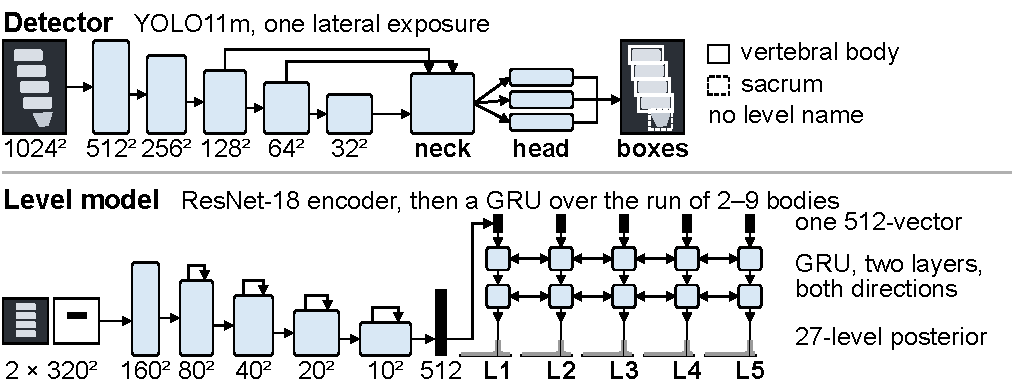
\includegraphics[width=4.35in]{figures/network_architecture.pdf}
\end{minipage}\hfill
\begin{minipage}[b]{2.25in}
  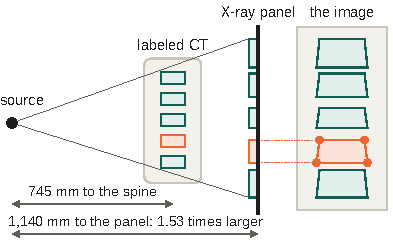
\includegraphics[width=2.25in]{figures/fig3b_projection.pdf}
\end{minipage}
\par\vspace{1pt}\noindent
\begin{minipage}{\linewidth}
\captionof{figure}{From the labeled CT to the C-arm image. (a) A YOLO11m detector boxes the bodies; a ResNet-18
encoder and a two-layer bidirectional GRU name each one among 27 levels. (b) At the device's geometry (0.1915\,mm per
pixel) the projection carries each labeled body of the CT, here a transitional one in orange, to its place on the
image.}
\end{minipage}\par\smallskip

\aim{Aim 3 (AI for Health): labeled 3-D structure into 2-D fluoroscopy, at low latency.} \emph{Data.} Physics
renders of CTSpinoPelvic1K, VerSe and TotalSegmentator CTs (7,045 standard and 1,482 transitional annotated frames)
and a device-styled corpus of 142 TotalSegmentator spines (12,730 entries); real frames of three devices: C-ArmLSpine
(149 cases; 617 lateral and 631 AP bodies whose truth is automatic, two CBCT labelers agreeing), DeepFluoro and COBRA
Elekta. \emph{Model} (Figure~3a): a YOLO11m detector boxes each body and the sacrum; a ResNet-18 encoder and a
bidirectional GRU name each body; a count from the sacrum checks the names, and the stack abstains where count and
shape disagree. New here: four corner keypoints per body, labeled for free by projecting each CT body's corners at
the device's geometry (Figure~3b). \emph{Closing the gap.} Physics renders randomized over devices' geometry and
spectra; real frames of two devices with the third held out; and a differentiable 3-D Gaussian X-ray renderer fitted
to each labeled CT, whose spectrum, scatter and detector response are learned until its renders stop being separable
from real frames, which today styled renders are 99 to 100\pct{} of the time. \emph{Cadaver set.} Two specimens from
WSU's Body Bequest Program are CT-scanned, then imaged AP and lateral at the protocol's lumbar and thoracic positions
on WSU's C-arm in Room 0312 Elliman (booked through DLAR, with OEHS dosimetry); a frame grabber records the C-arm's
video output, the set is sealed by hash before any model sees it, and the CT gives every frame its truth.
\emph{Preliminary results} (Figure~4, all held out by person): with no C-arm frame in training the level model names
96.4\pct{} of 617 lateral bodies on C-ArmLSpine but 43.7\pct{} of AP bodies, and the device's own frames, from other
patients, lift AP to 96.4\pct{}; count and shape together name 98.2\pct{} of the 1,009 bodies on frames that show the
sacrum, and a stop signal fires on 9.9\pct{} of 233 anchored frames, catching five of the six that err. Trained on two
other devices' real frames, the detector finds 80.5\pct{} of C-ArmLSpine's vertebrae at the 0.74 cross-device
operating point; no held-out cell met the pre-stated 97\pct{}. The stack's end-to-end latency has not been measured;
Aim 3 measures it first. \emph{H3:} 97\pct{} of vertebrae detected on the held-out device at 0.74, under 1\,s per
exposure on one H200, and every cadaver frame reported against its CT-derived truth.


\placefigure{\linewidth}{figures/fig4_results.pdf}{Held-out results with 95\pct{} Wilson intervals on the effective
sample size where the record gives one. (a) Exact level named on C-ArmLSpine, without and with the device's own frames in training. (b)
Vertebrae found on C-ArmLSpine, held out of detector training, at the 0.74 cross-device operating point, against the
pre-stated 97\pct{}; at 0.25 the two-device detector finds 90.6\pct{}.}

\subsection*{3. Evaluation: data, metrics and design}
{\footnotesize
\begin{tabularx}{\linewidth}{@{}p{0.3in}>{\raggedright\arraybackslash}X>{\raggedright\arraybackslash}X%
>{\raggedright\arraybackslash}p{1.45in}>{\raggedright\arraybackslash}p{1.55in}@{}}
\toprule
Aim & Data & Metrics & Design & Gate, written before the run\\
\midrule
1 & 40 tasks from the repository and Aim 3, each with its gate: 10 development, 30 sealed &
  pass rate; repairs per task; interventions; rule violations (a login-node run, a wrong QoS, a credential in a
  file); GPU-hours per pass &
  three arms, one model, one budget per task; three seeds; paired bootstrap over tasks &
  $\geq$80\pct{} pass on the 30 sealed tasks, 0 interventions, 0 violations; one shot passes under half\\
2 & 2027 cohort, 8 trainees in two waves \tbd{confirm}; the 2026 cohort (n = 16) as context &
  six-domain comfort before and after; days to first successful GPU job; tasks passed without a mentor; pull
  requests and abstracts &
  prospective cohort, the 2026 instrument, analysis plan registered before enrollment &
  all six domains improve (one-tailed Wilcoxon, $p<0.05$); median first GPU job within 7 days\\
3 & C-ArmLSpine, DeepFluoro and COBRA Elekta frames; the render banks; the sealed cadaver set &
  exact level per frame; vertebra and sacrum recall at 0.74; corner error (mm); Dice and IoU of the projected
  silhouette; latency per exposure (median, p95); abstention; render-to-real separability &
  leave-one-device-out; the cadaver set opened once, after code and weights are hashed &
  97\pct{} detection on the held-out device; under 1\,s per exposure on one H200; every cadaver frame reported
  against CT truth\\
\bottomrule
\end{tabularx}}

Frames cluster within cases, so every interval is Wilson on the effective sample size. The cadaver set is a sanity
test on real anatomy with CT truth, not a powered test; the powered tests are the held-out device and C-ArmLSpine, and
the laboratory's power analysis (35 persons with no error for a 90\pct{} lower bound) sets the R21's sample.

\subsection*{4. Expected outcomes, deliverables and timeline}
Within the award: (1) the agent, its benchmark and the three-arm report, under the MIT license with the tasks a
disclosure review clears; (2) the cohort's outcomes, pull requests and abstracts; (3) the paired CT and C-arm cadaver
set, deposited beside CTSpinoPelvic1K as the Body Bequest Program's terms allow, with the transfer and latency results
in a manuscript; (4) an FDA Pre-Submission; (5) NSF CAREER and NIH R21 submissions. \emph{Quarter 1:} agent version
1, benchmark sealed, IRB, recruitment, specimens and C-arm booked. \emph{Quarter 2:} benchmark run, wave 1 (months 4
to 7), cadaver imaging, latency and transfer results; Pre-Submission filed in April, so that FDA's written feedback,
due within 70 days, precedes the R21. \emph{Quarter 3:} CAREER (July 28), wave 2 (months 8 to 11), Gaussian
renderer. \emph{Quarter 4:} R21 (October 18), cadaver set opened, final report and AIDaS symposium. \emph{Risks.} An
agent not ready by month 4 starts wave 1 on the 2026 setup; a delayed specimen leaves the held-out device's frames as
the test; a transfer result under 97\pct{} becomes the R21's first aim; each task's budget caps its cost.

\vspace{2pt}
{\fontsize{7}{8.2}\selectfont
\begin{multicols}{2}
\raggedright
\textbf{References.}
[1] Furuya M, et al. Bone Joint J 2026;108-B(5):673-80.
[2] Mody MG, et al. Spine 2008;33(2):194-8.
[3] Groff MW, et al. World Neurosurg 2013;79(3-4):585-92.
[4] Bettis T, et al. Patient Saf Surg 2026. doi:10.1186/s13037-026-00508-9.
[5] Nakagawa T, et al. Tohoku J Exp Med 2017;242(3):223-8.
[6] Otake Y, et al. Phys Med Biol 2012;57(17):5485-508.
[7] Manbachi A, et al. Ann Biomed Eng 2018;46(10):1548-57.
[8] De Silva T, et al. Spine 2016;41(20):E1249-56.
[9] Open Spine Consortium. CTSpinoPelvic1K, release 11. Zenodo, doi:10.5281/zenodo.22797014.
[10] Jimenez CE, et al. SWE-bench: can language models resolve real-world GitHub issues? ICLR 2024.
[11] Cai Y, et al. Radiative Gaussian splatting for efficient X-ray novel view synthesis. ECCV 2024.
[12] Zha R, et al. R$^2$-Gaussian: rectifying radiative Gaussian splatting for tomographic reconstruction. NeurIPS
2024.
[13] OpenSpineConsortium: an open-source framework for medical student engagement in computational spine imaging
research. Cureus 2026;18(7):e112661.
\end{multicols}}

\clearpage

% ---------------------------------------------------------------- alignment page
\section*{AIDaS funding priority alignment}

\subsection*{Target agencies, programs and solicitations}
\begin{enumerate}[leftmargin=1.3em]
\item \textbf{NSF CAREER} (NSF 22-586; CISE, Division of Information and Intelligent Systems), PI Han. Research
  plan: Aim 1's gate-conditioned agent and Aim 3's 3-D-to-2-D learning; education plan: Aim 2's trainees.
  Deadline July 28, 2027, the fourth Wednesday of July; eligibility is judged at the deadline (untenured Assistant
  Professor, no earlier CAREER award) \tbd{the PI's tenure timing and earlier CAREER competitions}. If the PI is not
  eligible, the same plan goes to IIS's core programs (Future CoRe, NSF 25-543, Robust Intelligence).
\item \textbf{NIH R21 at NIBIB}: the reissued Trailblazer Award for New and Early Stage Investigators (forecast
  FOR-EB-26-001; the last notice, PA-25-169, expired May 8, 2026), or else NIBIB's Exploratory/Developmental
  Bioengineering Research Grant (EBRG, PAR-25-321) or the parent R21 (PA-25-304), both open through October 2027. Submission October 18, 2027, the
  standard October 16 falling on a Saturday, while the PI is still an Early Stage Investigator. Preliminary data: the
  cadaver set, the held-out-device result and the measured latency; FDA's Pre-Submission feedback shapes its
  validation aim.
\item \textbf{NSF CyberTraining} (NSF 23-520), a Pilot of up to \$300,000 over two years led by Co-PI Schwiebert:
  agent-assisted training of researchers on advanced computing, from Aim 2. Deadline January 20, 2028, the third
  Thursday of January; submitted in any case.
\item \textbf{NSF Smart Health} (SCH; the last solicitation, NSF 25-542, awaits its successor): the whole loop as a
  four-year project once NSF publishes the next call.
\end{enumerate}

\subsection*{Relevance to national science and technology priorities}
America's AI Action Plan (July 2025) asks for investment in AI-enabled science and, in its worker-first agenda, for
AI skills in the workforce, which Aim 2 builds in Michigan's medical trainees. Executive Order 14363 (November 2025) launches the Genesis Mission, which joins AI agents to national computing, and
NSF's Dear Colleague Letter 26-023 invites proposals to existing programs that support it, as NIH's Bio Genesis
Mission does for biomedicine. Aim 1 is that agenda at a university's scale: an agent that runs science on shared
computing and is held to verifiable gates. Executive Order 14303, Restoring Gold Standard Science (May 2025), and
OSTP's guidance of June 2025 ask agencies to promote pre-registration of study protocols and transparent reporting of
null results; every gate in this project is pre-registered by hash, and failed gates are reported. NIH's data
sharing policy and its Strategic Plan for Data Science 2025--2030 ask for data others can reuse, which CTSpinoPelvic1K
and the cadaver set are, and FDA's Q-Submission program gives Aim 3 a regulatory path within the award.

\subsection*{Team, expertise and roles}
The PI, a computer vision researcher who leads the Machine Perception Lab and publishes on 3-D Gaussian splatting and
neural implicit surfaces (CVPR 2025 and 2026, NeurIPS 2024), builds the agent and the 3-D-to-2-D model, including
the Gaussian X-ray renderer. The Co-PI, a high-performance computing researcher who accelerates scientific codes on
GPUs, builds the benchmark harness and the grid integration and leads the CyberTraining Pilot; the Co-PI and the
clinical collaborator have published four high-performance computing papers together (2021 to 2024). The clinical collaborator
holds the record this proposal builds on and runs the cohort, the IRB determination and the imaging session. The
part-time researcher of line A runs the benchmark, logs the measures and curates the cadaver set. Effort: PI
\tbd{\%}, Co-PI \tbd{\%}, in kind.

\subsection*{Timeline for external submission}
{\small
\begin{tabularx}{\linewidth}{@{}>{\raggedright\arraybackslash}p{1.95in}X@{}}
\toprule
When & Milestone\\
\midrule
January to March 2027 (months 1--3) & One-page concepts to the NSF IIS and NIBIB program officers; benchmark and gates
  sealed\\
April 2027 (month 4) & FDA Pre-Submission filed; written feedback due within 70 days\\
July 28, 2027 (month 7) & NSF CAREER submitted, with Aim 1's benchmark and Aim 3's leave-one-device-out results\\
October 18, 2027 (month 10) & NIH R21 submitted, with the cadaver set, the latency and FDA's feedback\\
December 2027 (month 12) & Project ends; AIDaS final report and symposium\\
January 20, 2028 (post-award month 1) & NSF CyberTraining Pilot submitted, Co-PI leading\\
2028 & R21 resubmission at the first standard date after its summary statement, under the parent R21 that replaces
  PA-25-304 \tbd{the reissued notice}; CAREER resubmission July 26, 2028, if eligible; SCH when NSF publishes it\\
\bottomrule
\end{tabularx}}

The CAREER and R21 meet the expectation of a federal proposal within 12 months of the project's end, and the
CyberTraining Pilot follows whatever their outcome; publications and proposals from the award acknowledge AIDaS.

\clearpage
% ---------------------------------------------------------------- budget page
\section*{Budget and justification}
{\small
\begin{tabularx}{\linewidth}{@{}l>{\raggedright\arraybackslash}p{2.35in}>{\raggedright\arraybackslash}X r@{}}
\toprule
Line & Item & Basis & Amount\\
\midrule
A & Part-time researcher, hourly & 520 h at \$15.00: Aim 1 180 h, Aim 2 160 h, Aim 3 180 h & \$7,800\\
A2 & Fringe on line A & FICA only, 7.65\pct{} & \$597\\
B1 & Two cadaver specimens, WSU Body Bequest Program & placeholder \$1,250 each \tbd{program fee} & \$2,500\\
B2 & Specimen CT, two scans & placeholder \$300 each \tbd{facility and rate} & \$600\\
B3 & C-arm session, Room 0312 Elliman, through DLAR & 4 h at a placeholder \$300 \tbd{DLAR rate} & \$1,200\\
B4 & Dosimetry and OEHS review for the session & placeholder \tbd{OEHS fee} & \$300\\
B5 & Frame grabber for the C-arm's video output & Magewell USB Capture AIO, list price & \$619\\
C1 & Claude Team Premium seats for the agents & 6 seats at \$15 a month for 12 months & \$1,080\\
C2 & Data management and storage & 2 TB of C\&IT hosted storage at \$400 per TB-year; Zenodo at no charge & \$800\\
D & FDA Pre-Submission: regulatory consultant & 10 h at \$300; FDA charges no fee & \$3,000\\
E & Anthropic AI for Science application & no fee; 8 of Aim 1's hours in line A & \$0\\
F & AIDaS symposium poster & 36 by 48 in at \$6 per sq ft & \$72\\
\midrule
& \textbf{Total requested} & & \textbf{\$18,568}\\
\bottomrule
\end{tabularx}}

\begin{itemize}[leftmargin=1.1em,itemsep=2pt]
\item \textbf{A, A2.} An hourly graduate student assistant where one is available, which is the call's graduate
  student support, or else a post-baccalaureate researcher; ten hours a week for 52 weeks. \$15.00 is Michigan's
  minimum wage from January 1, 2027 (MCL 408.934) \tbd{WSU's job category and scale}. Aim 1's hours are 360 runs
  at half an hour each; Aim 2's run the cohort's accounts and measures; Aim 3's are 100 hours curating the cadaver set
  (de-identifying, labeling, sealing by hash) and 80 running the leave-one-device-out and latency jobs. Temporary
  employees are not benefit-eligible, so the fringe is FICA alone (an enrolled student owes less). At \$18 an hour
  the total would be \$20,247, over the cap unless the hours fall to 507.
\item \textbf{B1 to B5.} A paired CT and C-arm set of the same anatomy exists in no public dataset, and it is the only
  test in which an X-ray's truth comes from a CT rather than a reader. The donor authorization of the Body Bequest
  Program permits de-identified images \tbd{the program's terms for public release}. The C-arm is WSU's own, in Room
  0312 Elliman, booked through DLAR: every user is enrolled in WSU's dosimetry program, with badges in the hands of
  DLAR's director at least 15 business days before the session, and completes OEHS's training form.
  The frame grabber records what the device shows, which is the deployment input; it takes SDI and composite video,
  since the C-arm's live output may be BNC \tbd{the C-arm's model and output}; at \$619 it is far under WSU's \$5,000
  capital threshold and becomes WSU property.
\item \textbf{C1, C2.} Anthropic's Team plan for scientists lets a verified PI add Premium seats at \$15 a month:
  four for the trainees, shared by the two waves, and two for the benchmark and development. The plan takes card
  payment only \tbd{P-card route and the PI's verification}; at Claude Pro's \$20 a month the line would be \$1,440.
  The dollars are list prices. The WSU grid's compute is free to WSU researchers and given in kind. Storage holds the
  render banks, the cadaver set and every benchmark run's logs for the award year; the data are deposited on Zenodo at
  its end.
\item \textbf{D.} FDA charges no fee for a Pre-Submission filed in 2027 (a fee is proposed only from fiscal year
  2028); the consultant, at a mid-level regulatory rate, reviews a package the PI writes (device description,
  intended use, proposed testing), so that FDA's written feedback reaches the R21.
\item \textbf{E, F.} AI for Science awards up to \$20,000 in API credits for six months and charges nothing to apply;
  credits would add benchmark seeds. Presenting at an AIDaS symposium is an award expectation; the poster is printed
  at the School of Medicine's Medical Communications.
\item \textbf{Not requested.} PI and Co-PI salary, travel, tuition, equipment and indirect costs \tbd{confirm AIDaS
  applies no F\&A}.
\item \textbf{Allowability and dependencies.} Lines A (as graduate student support), C1 and C2 fall under the call's
  allowable headings and alone total \$10,277, above the \$10,000 floor. Lines B, D and F are research costs the AIDaS
  office is asked to confirm before submission. B2 to B5 depend on B1, since without a specimen there is nothing to
  scan or image. Without B the request is \$13,349 and Aim 3 tests on the held-out device's frames, its 100 cadaver
  hours moving to extra benchmark seeds; without B and D it is \$10,349; without B, D and F, \$10,277.
\end{itemize}

\clearpage
% ---------------------------------------------------------------- biosketches
% Each biosketch is placed when its file is present; the placeholder page stands only when neither is.
\newif\ifanybiosketch
\IfFileExists{biosketch_han.pdf}{\anybiosketchtrue}{}
\IfFileExists{biosketch_schwiebert.pdf}{\anybiosketchtrue}{}
\ifanybiosketch
  \IfFileExists{biosketch_han.pdf}{\includepdf[pages=-]{biosketch_han.pdf}}{}
  \IfFileExists{biosketch_schwiebert.pdf}{\includepdf[pages=-]{biosketch_schwiebert.pdf}}{}
\else
\section*{Biosketches}
The two investigators' biosketches, two pages each in NSF format, follow this page in the submitted PDF. Put
\texttt{biosketch\_han.pdf} and \texttt{biosketch\_schwiebert.pdf} beside \texttt{main.tex} and compile again, and
they replace this page.
\fi

\end{document}
